\documentclass{article}
\usepackage[utf8]{inputenc}

\title{Homework No.4 - Model Wing Simulation Example from courses.ansys.com}
\author{Osamu Katagiri-Tanaka : A01212611}
\date{\today}

% import math symbols
\usepackage{amsmath, esint}
\usepackage{cancel}

% import code snippets
\usepackage{listings}
\usepackage{xcolor}
\definecolor{codegreen}{rgb}{0,0.6,0}
\definecolor{codegray}{rgb}{0.5,0.5,0.5}
\definecolor{codepurple}{rgb}{0.58,0,0.82}
\definecolor{backcolour}{rgb}{0.99,0.99,0.96}
\lstdefinestyle{mystyle}{
  backgroundcolor   = \color{backcolour},
  commentstyle      = \color{codegreen},
  keywordstyle      = \color{magenta},
  numberstyle       = \tiny\color{codegray},
  stringstyle       = \color{codepurple},
  basicstyle        = \ttfamily\small,
  breakatwhitespace = false,
  breaklines        = true,
  captionpos        = b,
  keepspaces        = true,
  numbers           = left,
  numbersep         = 5pt,
  showspaces        = false,
  showstringspaces  = false,
  showtabs          = false,
  tabsize           = 2
}
\lstset{style=mystyle}

% import hyperlinks
\usepackage{hyperref}
\hypersetup{
  colorlinks = true,
  linkcolor  = red,
  filecolor  = red,
  citecolor  = red,
  urlcolor   = red
}

% import continuous lists
\usepackage{enumitem}

% format margins and paper size
\usepackage{geometry}
\geometry{
	paper         = a4paper, % Change to letterpaper for US letter
	inner         = 2.5cm,   % Inner margin
	outer         = 2.5cm,   % Outer margin
	bindingoffset = 0.5cm,   % Binding offset
	top           = 1.5cm,   % Top margin
	bottom        = 1.5cm    % Bottom margin
}

% import figure handler
\usepackage{graphicx}

% import references handler
\usepackage[
  style     = ieee,         % references format style
  backend   = biber,        % choose the processing program
  natbib    = true,         % enable additional reference formats
  citestyle = numeric-comp, % enable multiple citations
  sortcites = true,         % sort references in multiple citations
  sorting   = nyt           % sort the reference table
]{biblatex}
\addbibresource{references.bib}

% Note that ‘d’ in the differential is conventionally set in roman.
\newcommand{\ud}{\,\mathrm{d}}

% Paragraph spacing
\setlength{\parskip}{0.2cm}           % spacing between paragraphs
\renewcommand{\baselinestretch}{1.25} % spacing between lines

\begin{document}

\maketitle

\section{Problem Statement}

Ansys' simulation example is to analyse low-speed air flow corresponding to take-off and landing conditions over a mock-up aircraft wing in a wind tunnel test set-up. Along with analyses of lift and drag generated by the wing. The required Mesh file and associated case \& data files were downloaded from \href{https://ansys13.ansys.com/AnsysInnovationCourses/FBU/Course%205%20-%20Dimensional%20Analysis%20and%20Similarity/Simulation%20Example%20-%20Model%20Wing/Model-Wing%20-%20Simulation%20Files.zip}{Ansys' website}. 

The model consists of a mock-up wing mounted at $5^\circ$ angle of attack inside a wind tunnel for testing with the following characteristics:

\begin{itemize}
  \item Test section dimensions: $16.96 \textrm{m} \times 6.8 \textrm{m} \times 6.11 \textrm{m}$ $(\textrm{L} \times \textrm{W} \times \textrm{H})$
  \item Wing span: $1.8 \textrm{m}$
  \item Wing reference chord: $0.665 \textrm{m}$
  \item Wing platform area: $1.0942 {\textrm{m}}^2$
\end{itemize}

The domain consists of two fluid region filled with air, named as ``Wind tunnel test section" and ``Wing nearfield". See Figure \ref{img:fluidRegions}. The inlet velocity is $\displaystyle 68 \frac{\textrm{m}}{\textrm{s}}$, which corresponds to Mach $0.2$. Effects of air compressibility are negligible when the mach number is less than $0.3$. Therefore, the air is at standard sea level conditions and assumed to be incompressible $\displaystyle \left( \rho_{air} = 1.225 \frac{\textrm{Kg}}{{\textrm{m}}^3} \textrm{ and } \mu_{air} = 1.7894 \times 10^{-5} \frac{\textrm{Kg}}{\textrm{m s}} \right)$.

\begin{figure}[h!]
	\centering
	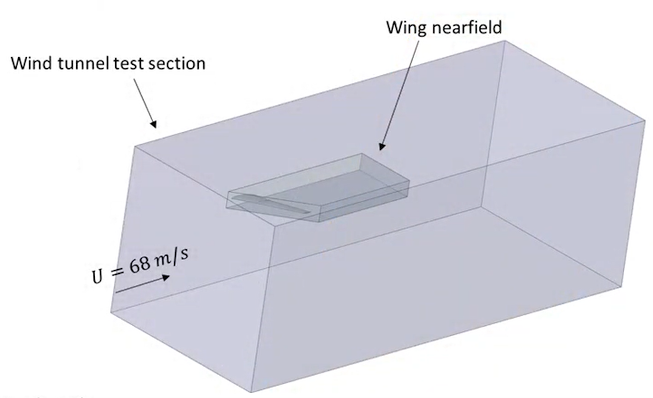
\includegraphics[width=0.75\textwidth]{./img/fluidRegions.png}
	\caption{Problem Statement - Fluid Regions : adapted from \cite{ANSYSmodelWing}}
	\label{img:fluidRegions}
\end{figure}

The Reynolds number based on the reference chord is $Re = 3.0 \times 10^6$, implying that the flow over the wing is fully turbulent. The air entering the tunnel is smooth with very little turbulence. As shown in Figure \ref{img:boundaryConditions}, the boundary conditions are as follows:

\begin{itemize}
  \item inlet: velocity inlet
  \item outlet: pressure outlet
  \item side and mounting walls: slip walls
  \item wing: no-slip wall
\end{itemize}

A steady state simulation is to be done using the pressure-based coupled solver in Ansys Fluent.

\begin{figure}[h!]
	\centering
	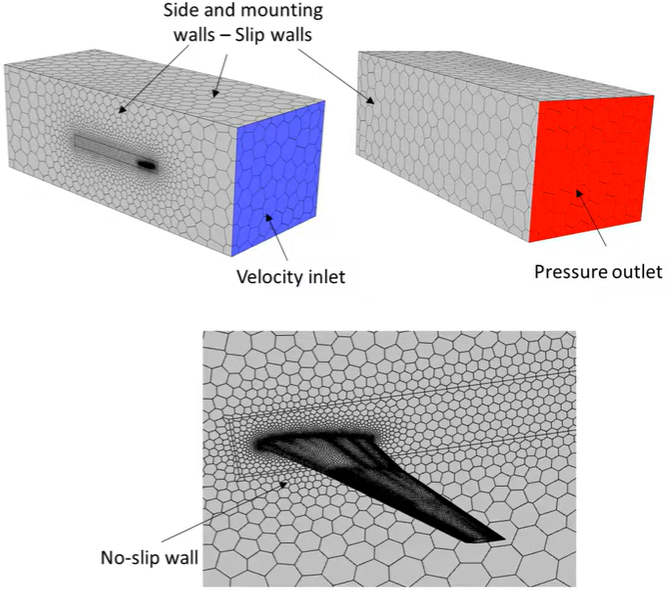
\includegraphics[width=0.75\textwidth]{./img/boundaryConditions.png}
	\caption{Problem Statement - Boundary Conditions : adapted from \cite{ANSYSmodelWing}}
	\label{img:boundaryConditions}
\end{figure}

\section{Simulation \& Results}

First step is to read the mesh file, also known as the ``wing model" by doing: $\textrm{FILE} \rightarrow \textrm{READ} \rightarrow \textrm{MESH}$

\begin{center}
  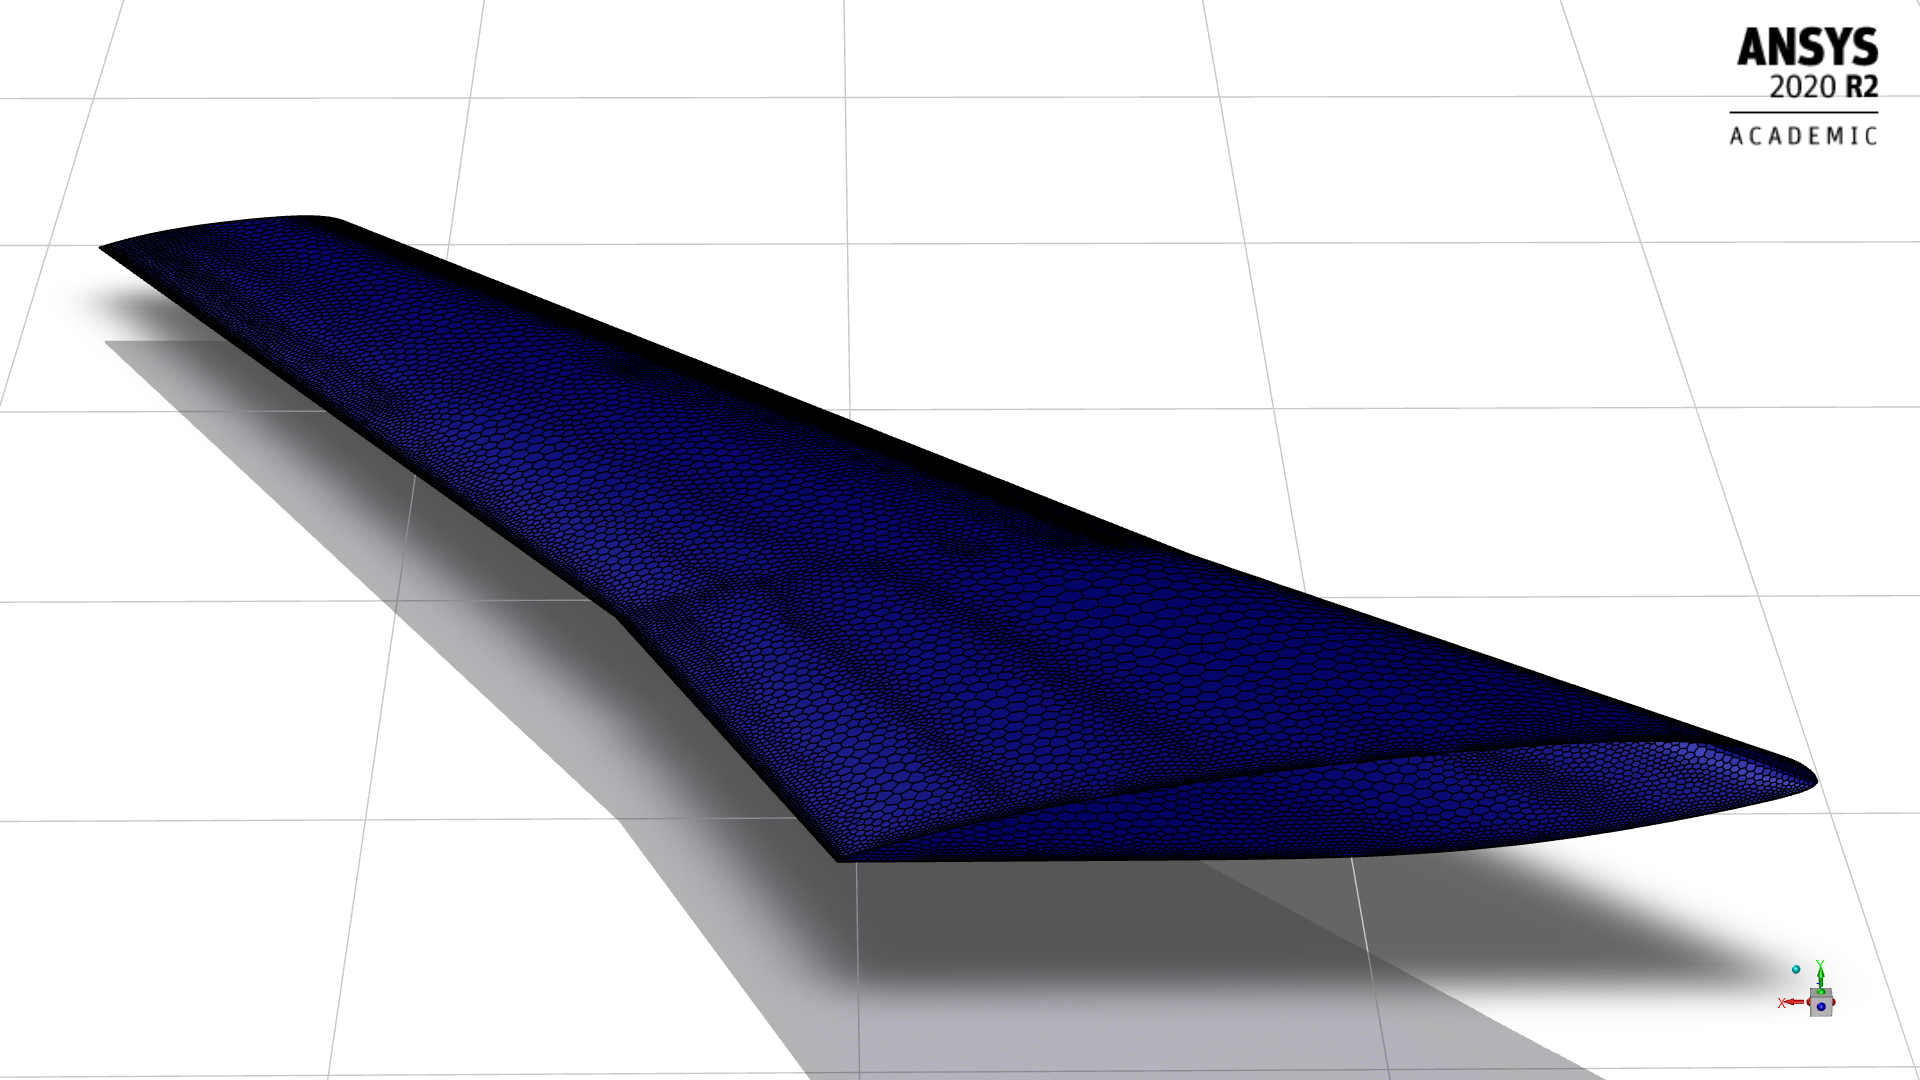
\includegraphics[scale=0.20]{./img/mesh.png}
\end{center}

Step two is to set-up the physics by opening the $\textrm{PHYSICS}$ tab. Under the $\textrm{REFERENCE VALUES...}$ menu, the wing properties (listed in the Problem Statement section) are specified.

\begin{center}
  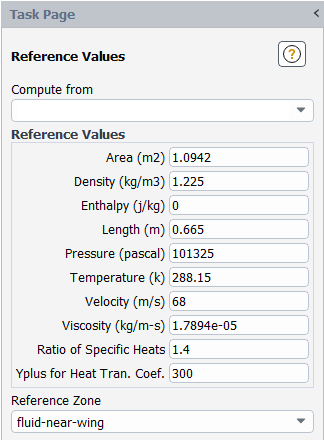
\includegraphics[scale=0.60]{./img/referenceValues.png}
\end{center}

Under the $\textrm{ZONES}$ menu, the boundary conditions are specified as depicted in the Problem Statement section. 

\begin{center}
  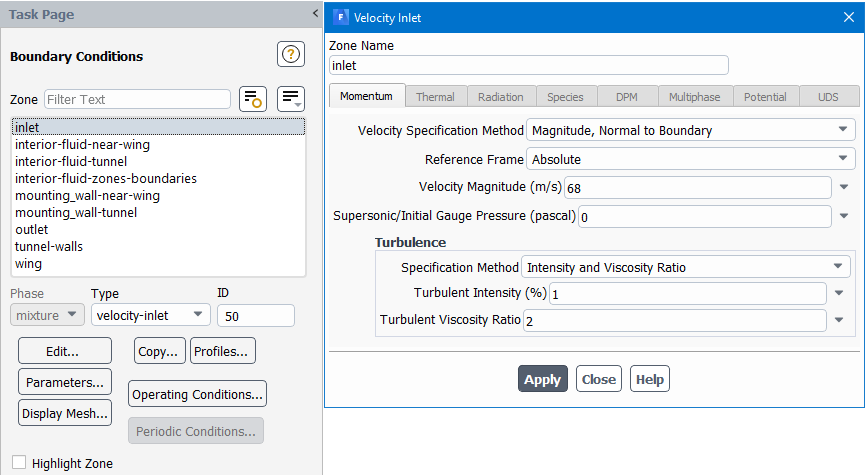
\includegraphics[scale=0.60]{./img/inletBoundaryCondition.png}
\end{center}

Once the model is initialized and solved, the results can be visualized as \emph{contours} and \emph{path-lines}

\begin{center}
  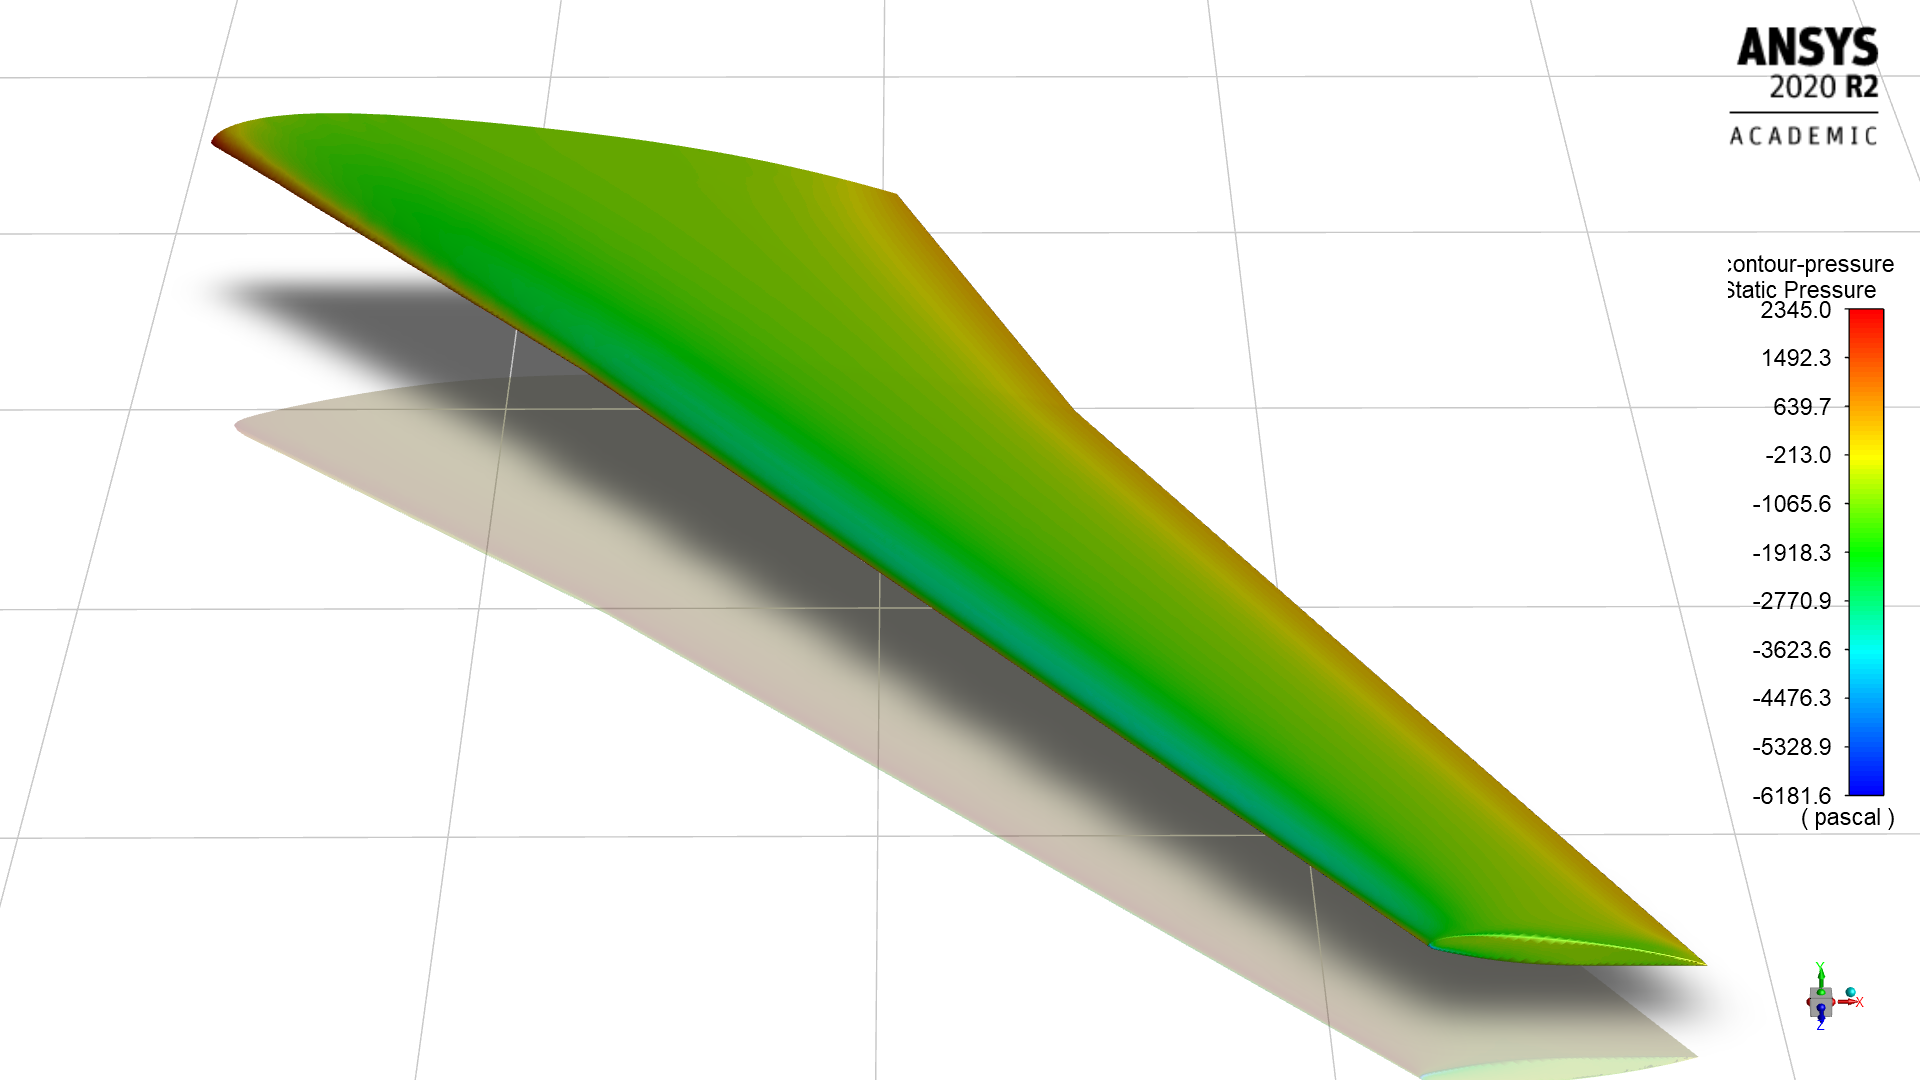
\includegraphics[scale=0.20]{./img/pressure.png}
\end{center}

\begin{center}
  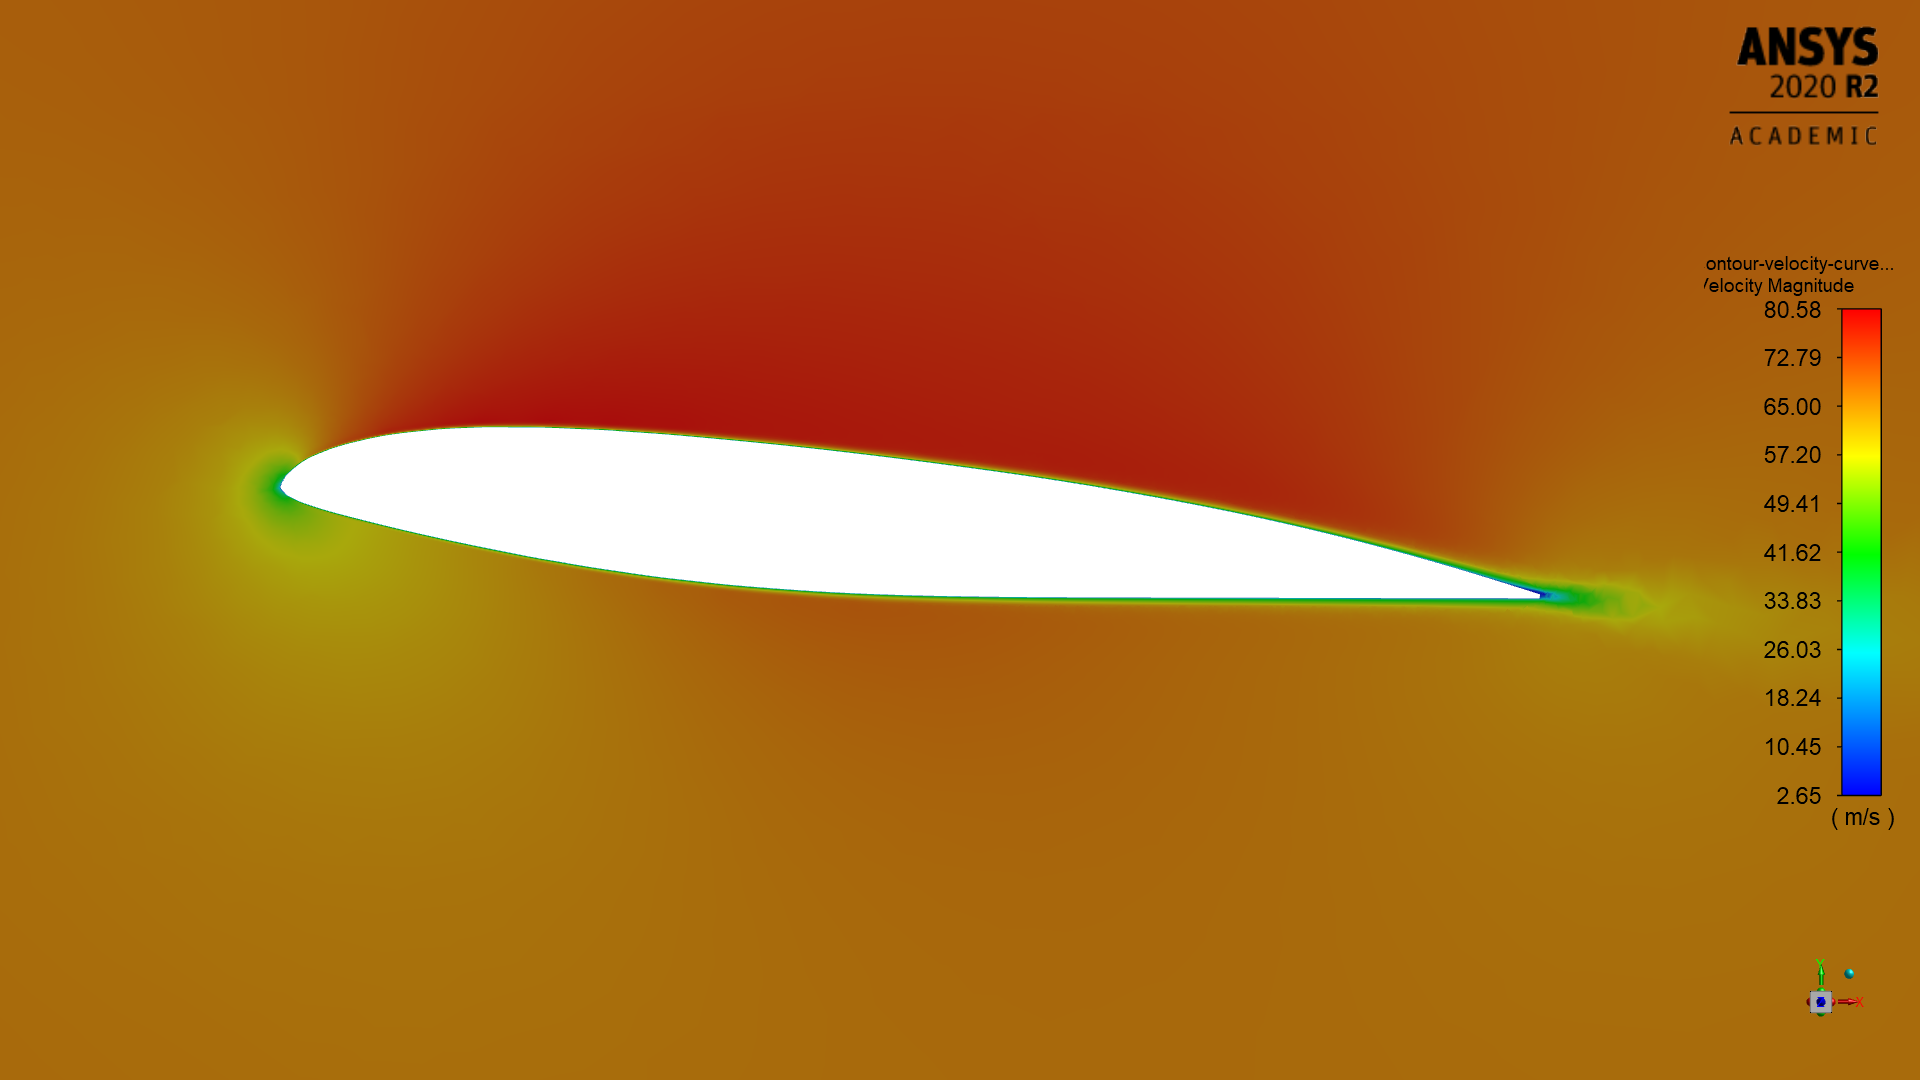
\includegraphics[scale=0.20]{./img/velocity_curvatureProfile.png}
\end{center}

\begin{center}
  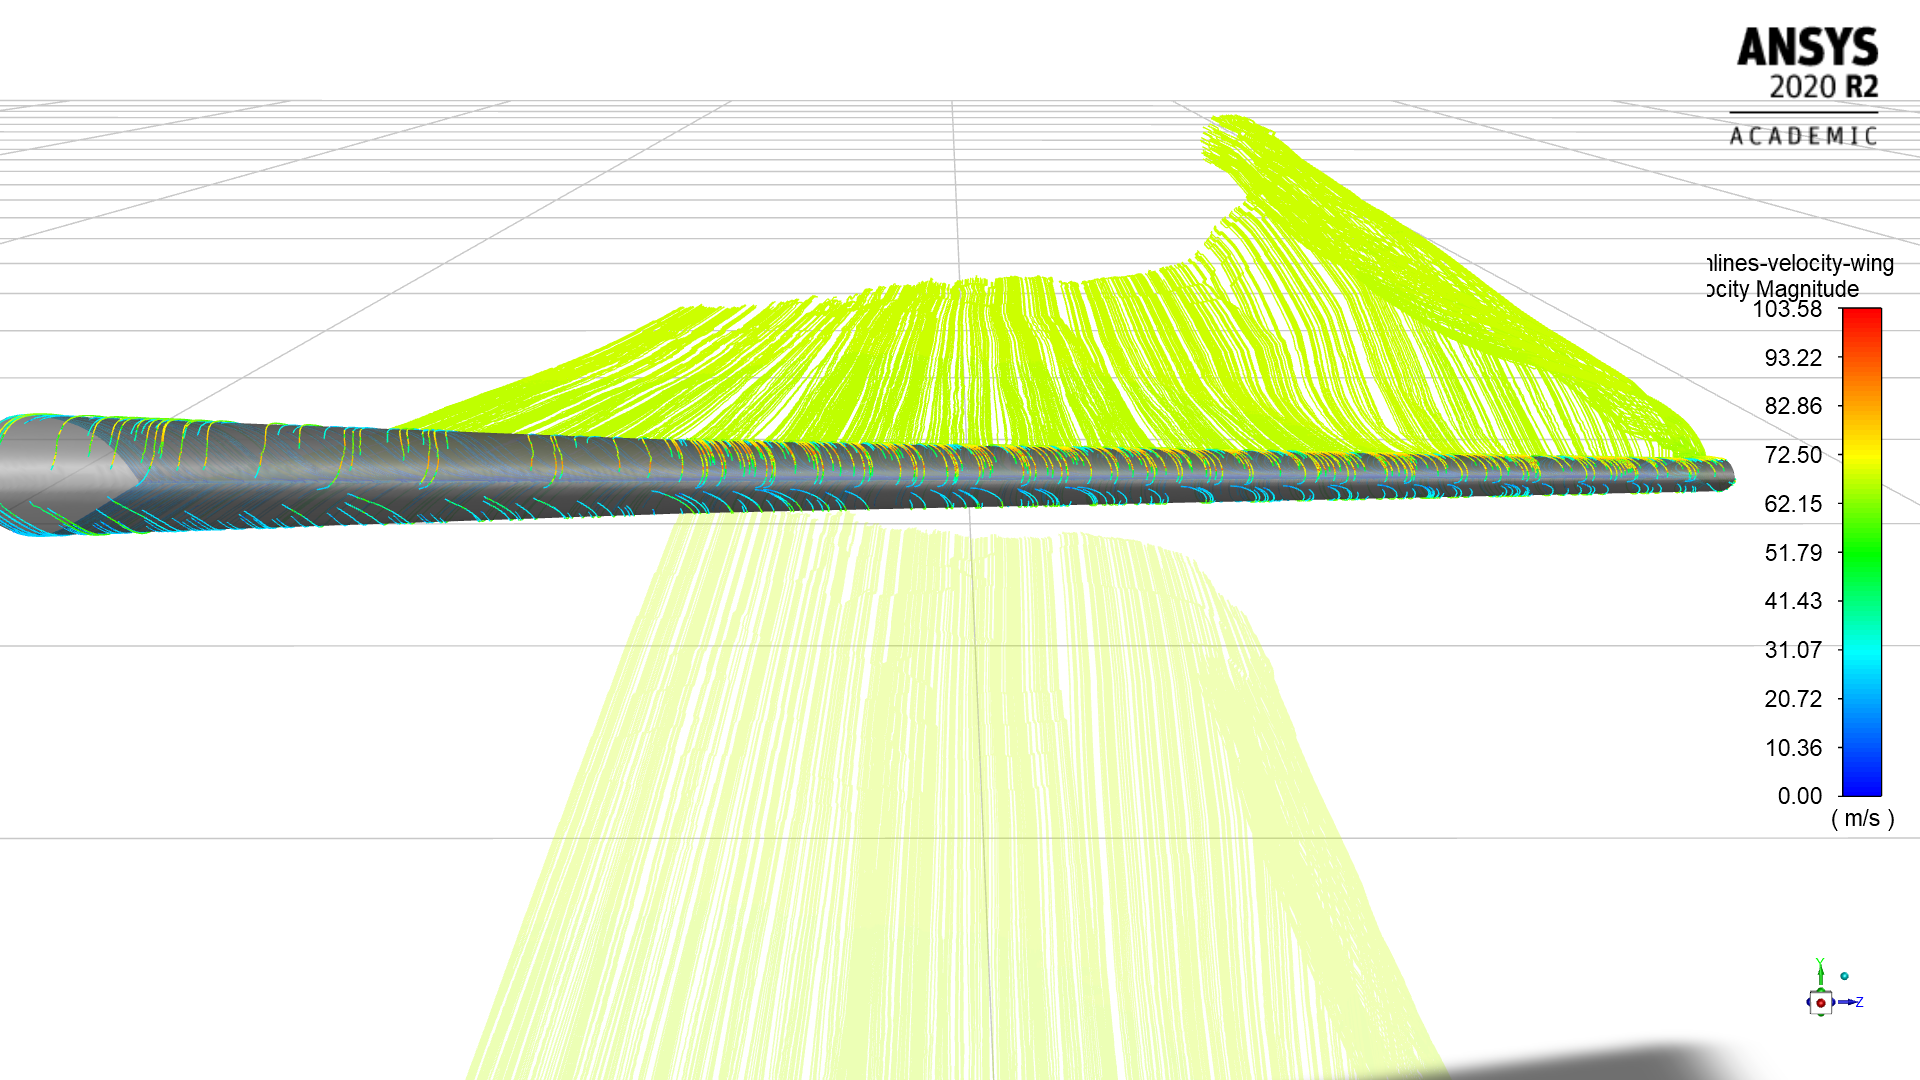
\includegraphics[scale=0.20]{./img/velocitypathlines_front.png}
\end{center}

\begin{center}
  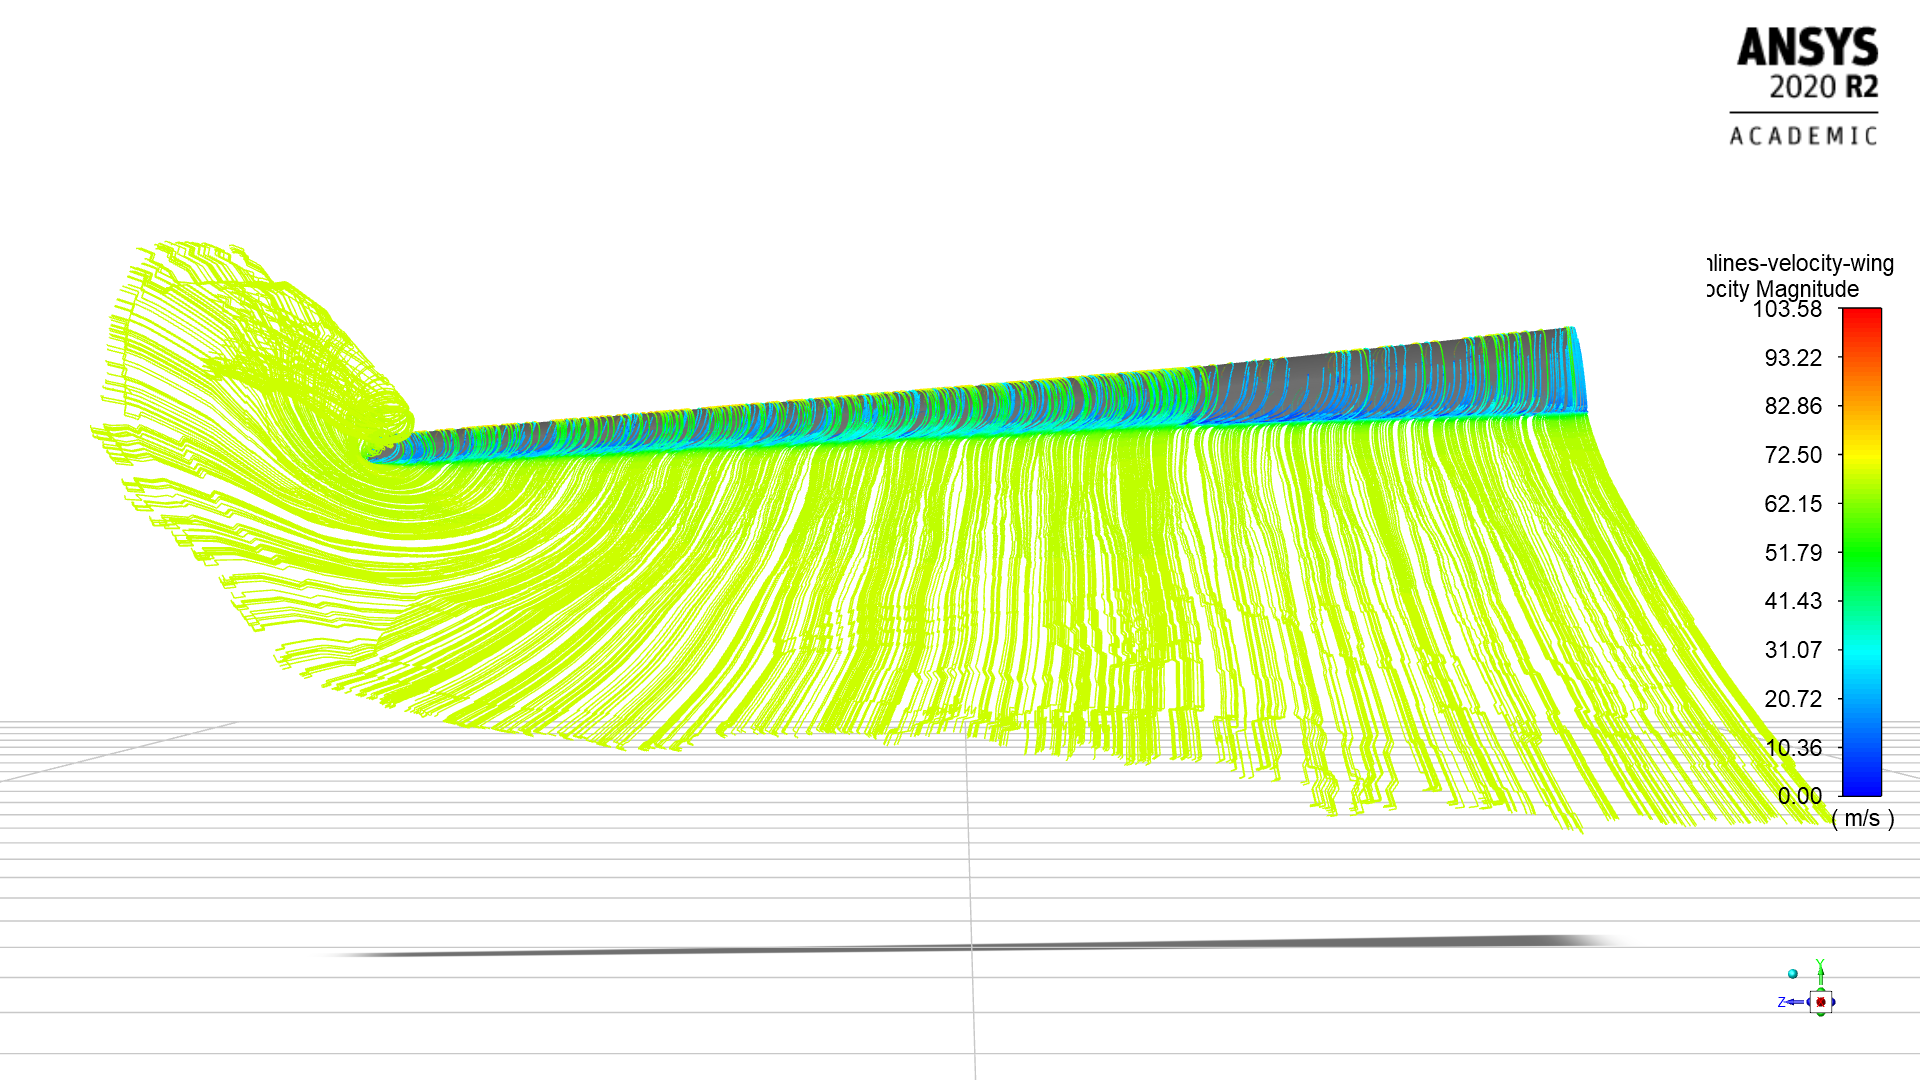
\includegraphics[scale=0.20]{./img/velocitypathlines_back.png}
\end{center}

\printbibliography[title={References}]
\end{document}
